\chapter{Introducción}
\label{chap:introduccion} 
En este primer capítulo de la memoria se van a explicar los conceptos clave entorno a los cuales se ha desarrollado este Trabajo de Fin de Grado. Entender qué son la robótica y las tecnologías web y por qué son importantes es fundamental, ya que la combinación de ambos conceptos ha dado lugar a la docencia robótica. \newline

Por otro lado, en este capítulo también se va a introducir el concepto de motor de físicas, ya que una importante parte del trabajo se ha basado en la generación de un motor de físicas complementario que permite recrear los movimientos realizados por los robots del entorno web de \textit{Kibotics} con un mayor realismo. \newline

\section{Robótica}
La robótica es la ciencia que estudia la creación de máquinas automatizadas capaces de recrear comportamientos humanos o animales en función del software que lleven incorporados. Estas máquinas son las que se denominan robots. \newline


Haciendo un breve repaso de la historia de los robots, cabe destacar que desde el 85 a.C. ya se empezaron a crear los primeros robots en la Antigua Grecia. En esa época la creación de robots se basaba en el intento de replicar personas por medio de máquinas. De hecho, esas máquinas ni siquiera se denominaban robots. El termino robot fue acuñado en 1920 por Karel Capek como homenaje a su obra teatral Rossum's Universal Robots, que trataba de una empresa encargada de fabricar humanos artificiales para facilitar la realización de tareas a los trabajadores de las fábricas. Así, la palabra Robot procede de Robbota, que en checo significa trabajo forzado o servidumbre\footnote{https://revistaderobots.com/robots-y-robotica/que-es-la-robotica/}. \newline


El primer robot del que se tiene contancia es el \textit{Elektro}. Fue construido en 1937 y se le conoce como \textit{el primer robot de la historia}. Este robot representaba a un humano de 2 metros de altura y 120 kg de peso. Era capaz de recrear movimientos humanos como caminar y de comunicarse utilizando hasta 700 palabras\footnote{\textit{Ibidem}}. Posteriormente, George Charles Devol creó el primer robot industrial en 1948. Por ello, George Charles Devol es considerado el inventor de la robótica. Junto a Joseph F. Engelberger, creó la empresa Unimation, que fue la responsable de la creación de gran parte de los primeros robots industriales de la historia\footnote{\textit{Ibidem}}.\newline

Hoy en día, los robots están presentes prácticamente en cualquier ámbito de la vida de cualquier persona. Ya se han creado robots capaces de recrear casi cualquier actividad realizada por el ser humano o que nos facilita la realización de las mismas. Algunos de los robots más populares en la actualidad son lo siguientes. En la Figura \ref{fig:EjemplosRobots} se ofrece una representación gráfica de ellos.
\begin{itemize}
\item Robots que se encargan de la limpieza del hogar (por ejemplo, Roomba).
\item Robots sociales encargados de hacer compañía (por ejemplo, Pepper).
\item Robots de cocina capaces (por ejemplo, Thermomix).
\item Robots especialistas en labores de rescate (por ejemplo, Atlas).
\item Drones (por ejemplo, Tello).
\item Coches autónomos (por ejemplo, Tesla).
\end{itemize} 

\begin{figure}[!tbp]
  \begin{subfigure}[b]{0.4\textwidth}
    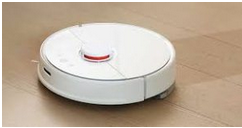
\includegraphics[width=\textwidth, height=\textwidth]{roomba.png}
    \caption{Roomba}
  \end{subfigure}
  \hfill
  \begin{subfigure}[b]{0.4\textwidth}
    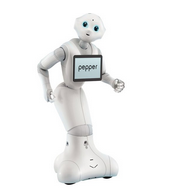
\includegraphics[width=\textwidth, height=\textwidth]{pepper.png}
    \caption{Pepper}
  \end{subfigure}
    \hfill
  \begin{subfigure}[b]{0.4\textwidth}
    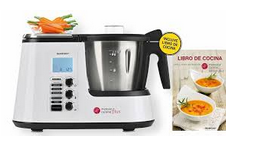
\includegraphics[width=\textwidth, height=\textwidth]{thermomix.png}
    \caption{Thermomix}
  \end{subfigure}
    \hfill
  \begin{subfigure}[b]{0.4\textwidth}
    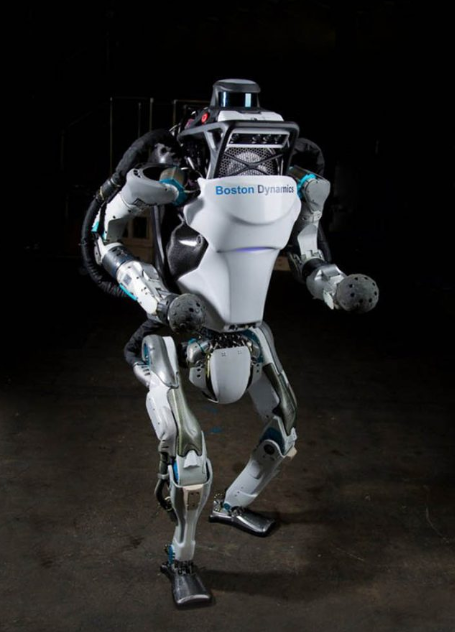
\includegraphics[width=\textwidth, height=\textwidth]{atlas.png}
    \caption{Atlas}
  \end{subfigure}
      \hfill
  \begin{subfigure}[b]{0.4\textwidth}
    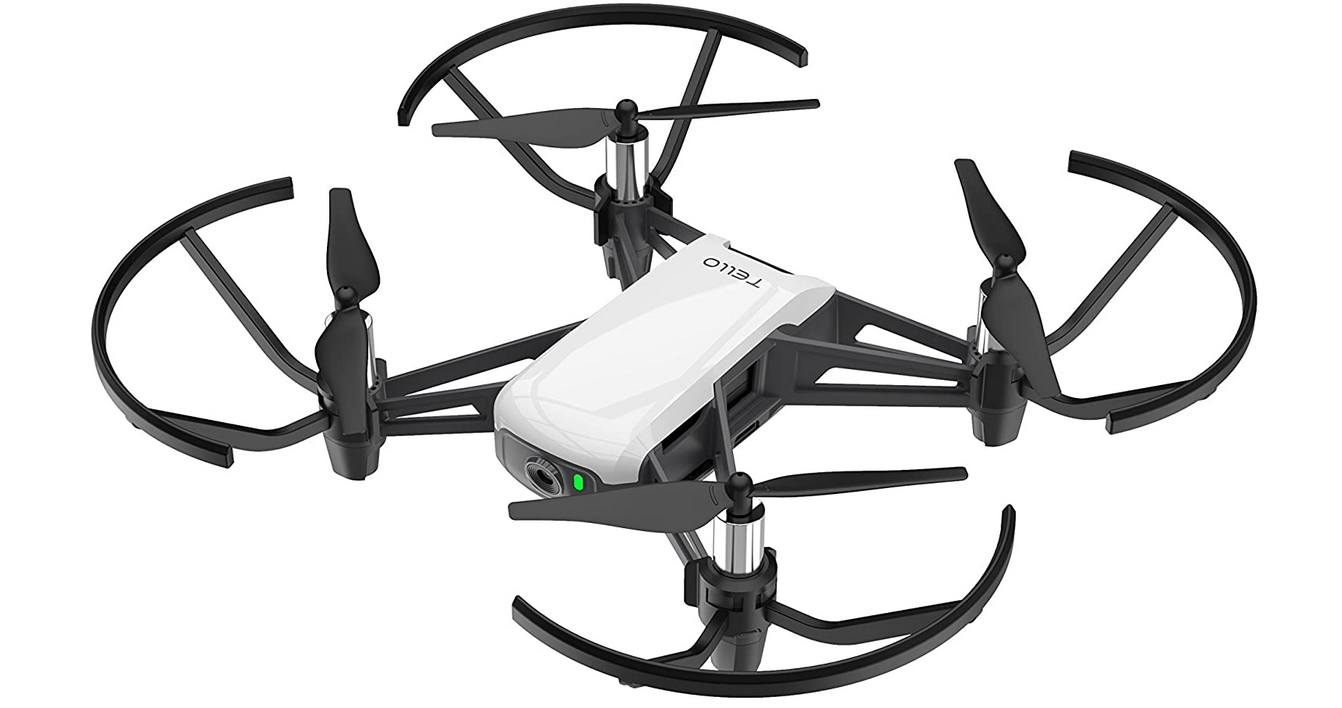
\includegraphics[width=\textwidth, height=\textwidth]{drone.png}
    \caption{Tello}
  \end{subfigure}
      \hfill
  \begin{subfigure}[b]{0.4\textwidth}
    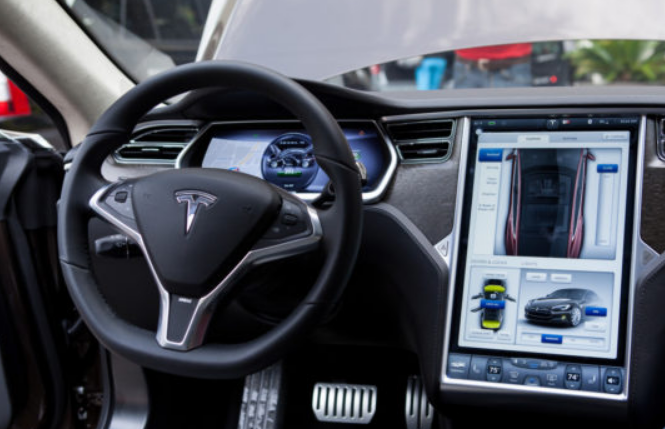
\includegraphics[width=\textwidth, height=\textwidth]{tesla.png}
    \caption{Tesla}
  \end{subfigure}
\caption{Ejemplos de robots en la actualidad}
\label{fig:EjemplosRobots}
\end{figure}


\section{Tecnologías web}
Las tecnologías web están en continúo desarrollo. Actualmente, existen tecnologías web tanto en el lado del cliente como en el lado del servidor. La idea de esta separación es marcar las diferentes partes de un sistema software para poder controlarlo de una forma más eficaz. Por este motivo, el frontend recoge los datos y el backend los procesa. \newline


Por un lado, el frontend engloba todas aquellas tecnologías web del lado del cliente que se encargan de recopilar los datos. Principalmente, existen tres tecnologías de frontend: \textit{HTML, CSS} y \textit{JavaScript}. Estas tres tecnologías permiten al usuario interactuar con el sevidor web, utilizando un navegador como intérprete. Por otro lado, el backend se encarga del almacenamiento de información en bases de datos, gestión de servidores y servir las vistas de las páginas web seleccionadas por el desarrollador en el lado del cliente. En el backend, el número de tecnologías es mucho más extenso. La programación backend incluye lenguajes como \textit{PHP, Python, .NET o Java }y las bases de datos sobre las que se trabaja pueden ser \textit{SQL, MongoDB o MySQL}. Todas estas tecnologías web permiten implementar comportamientos determinados de las aplicaciones web en el servidor. En la Figura \ref{fig:tecnologias} se muestra un esquema de la división de las tecnologías web entre ambos planos. \newline

\begin{figure}[h!]
    \centering
    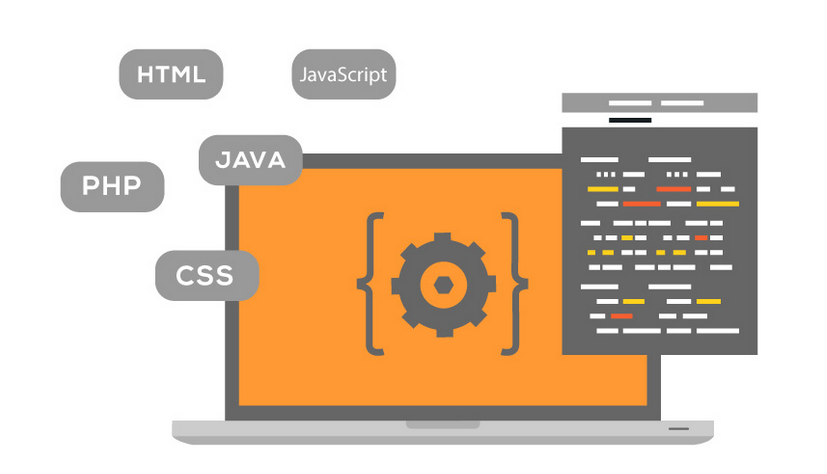
\includegraphics[scale=0.4]{tecnologias.png}
    \caption{Tecnologías web en el lado del cliente y del servidor \footnotemark}
    \label{fig:tecnologias}
\end{figure}
\footnotetext{https://www.ingeniovirtual.com/conceptos-basicos-sobre-tecnologias-de-desarrollo-web/}
  
\subsection{Tecnologías web en el lado del cliente}
Las tres tecnologías web del frontend que permiten la interacción entre usuario y servidor web son las siguientes:
\begin{itemize}
    \item \textbf{HTML:} es un lenguaje de marcado que permite diferenciar los contenidos y definir la estructura de un sitio web. Permite dividir una página web en diferentes secciones: títulos, texto, imágenes, pie de página, etc. Es la base de toda página web.
    \item \textbf{CSS}: es un lenguaje de hojas de estilo que permite modificar la apariencia de una página web.
    \item \textbf{JavaScript:} es un lenguaje de programación interpretado que permite definir el comportamiento de una página web (por ejemplo, al hacer click en un enlace). Por ello, gracias a JavaScript el usuario puede interaccionar con la página web.
\end{itemize}

\subsection{Tecnologías web en el lado del servidor}
Uno de los lenguajes más utilizados en la programación del backend es el lenguaje \textit{JavaScript}. \textit{JavaScript} se creó para su uso en el frontend en un principio; sin embargo, gracias al motor \textit{NodeJS}, este lenguaje puede ser interpretado en el lado del servidor sin necesidad de un navegador. \newline


El código \textit{JavaScript}  del cliente y el servidor es independiente el uno del otro. Sin embargo, resulta de especial interés el hecho de que se pueda desarrollar código en un mismo lenguaje tanto en el frontend como en el backend por las facilidades y reducción de tiempos y esfuerzo que esto supone para los desarrolladores. \newline
 
Se puede utilizar el mismo lenguaje en todos los contextos del desarrollo: en el cliente de escritorio con DOM, en el cliente móvil con \textit{Cordova o React Native}, en el servidor con \textit{Node.js} o en la base de datos con \textit{MongoDB}. En cuanto a la tecnología empleada, las herramientas que se utilizan en el backend son principalmente: editores de código, compiladores, depuradores de código y gestores de bases de datos. \newline

La comunicación entre cliente y servidor se realiza utilizando el protocolo \textit{HTTP} (protocolo de transferencia de hipertexto). Este protocolo funciona mediante la emisión de una serie de peticiones y respuestas entre el cliente y el servidor usando diferentes métodos. Existen numerosos métodos \textit{HTTP}, pero los más comunes son los siguientes\footnote{https://developer.mozilla.org/es/docs/Web/HTTP/Methods}:

\begin{itemize}
    \item \textbf{GET}: solicitud de datos de un recurso concreto.
    \item \textbf{PUT}: reemplazo de las representaciones actuales del recurso de la petición.
    \item \textbf{POST}: envío de datos a un recurso concreto, normalmente provocando el cambio de estado del servidor.
    \item \textbf{DELETE}: eliminación de un recurso.
     \item \textbf{HEAD}: solicitud de datos de un recurso concreto tal y como ocurre con el método \textit{GET}, pero la respuesta no incluye cuerpo.
\end{itemize}

\begin{figure}[h!]
    \centering
    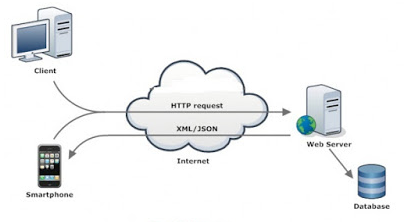
\includegraphics[scale=1]{http.png}
    \caption{Ejemplo de una interacción \textit{HTTP} \footnotemark}
    \label{fig:http}
\end{figure}
\footnotetext{http://dsanchezzz.blogspot.com/2015/10/rest.html}

\section{Docencia robótica}
En la intersección entre la robótica y las tecnologías web se encuentra la docencia robótica. La docencia robótica tiene como objetivo el acercamiento a las tecnologías web de última generación que permiten el desarrollo software para la creación de robots desde edades tempranas. \newline


Hoy en día, el plan de educación que se imparte en colegios e institutos no hace hincapié en la enseñanza de estas tecnologías, por lo que los niños no se encuentran especialmente motivados en el desarrollo de software robótico ya que desconocen su uso y posibilidades. En consecuencia, especialmente en los últimos años, han surgido algunas plataformas dedicadas a la docencia robótica que se encargan de impartir cursos de iniciación a la robótica desde edades muy tempranas para conseguir que los niños se sientan atraídos por esta rama desde el principio y aprendan a pensar como verdaderos programadores desde muy pequeños. \newline



Un ejemplo de estas plataformas que se comentan es el de \textit{Lenobotics}.  \textit{Lenobotics} es un programa que se encarga de impartir cursos de robótica en centros educativos para desarrollar las habilidades cognitivas de los niños que resultan necesarias para la programación\footnote{https://lenobotics.com/}. \newline

\begin{figure}[h!]
    \centering
    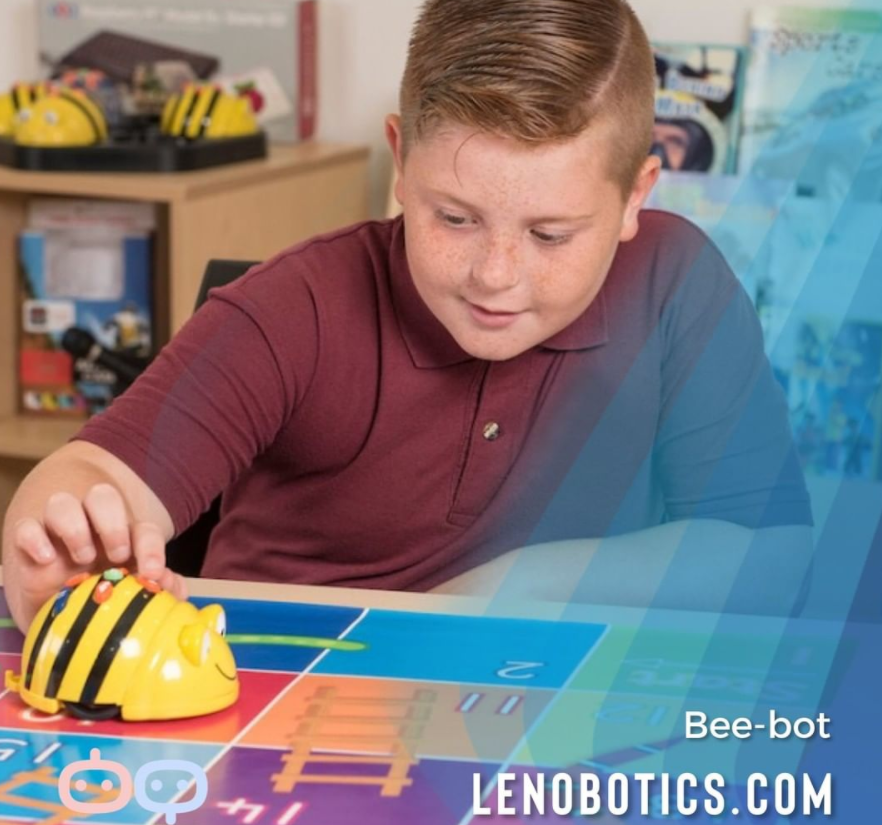
\includegraphics[scale=0.55]{lenobotics.PNG}
    \caption{Aprendizaje de programación robótica con \textit{Lenobotics}}
    \label{fig:lenobotics}
\end{figure}


Por su parte, \textit{LEGO education}  también ofrece a los más pequeños la posibilidad de iniciarse en la robótica a través de sus kits de robótica. Estos kits permiten aprender unas primeras nociones de electrónica, robótica y programación\footnote{https://education.lego.com/es-es}. \newline

\begin{figure}[h!]
    \centering
    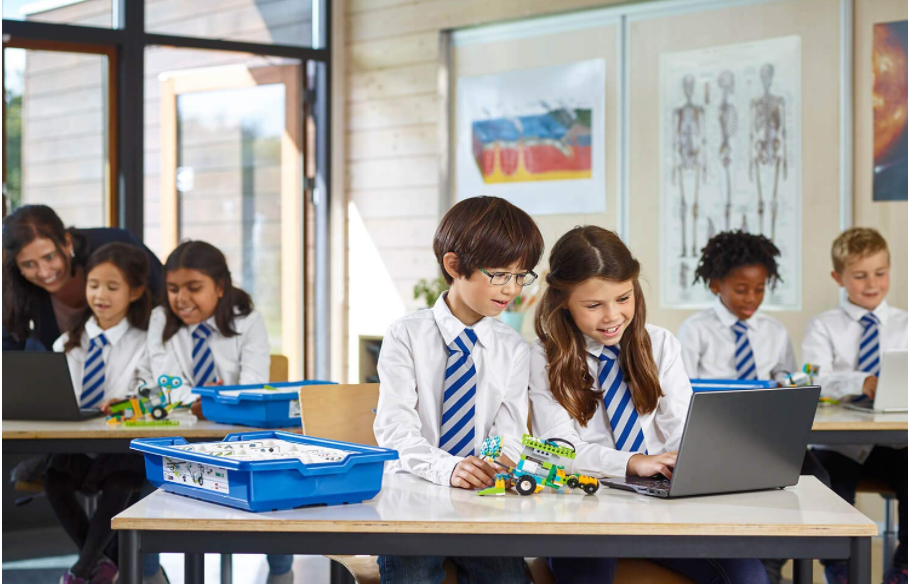
\includegraphics[scale=0.7]{lego.PNG}
    \caption{Aprendizaje de programación robótica con \textit{LEGO education}}
    \label{fig:lego}
\end{figure}

El presente trabajo se va a centrar en la plataforma \textit{Kibotics}\footnote{https://kibotics.org/}. \textit{Kibotics} es un entorno web para docencia en robótica y programación que permite a niños y adolescentes aprender programando. Esto quiere decir que \textit{Kibotics}  apuesta por una enseñanza puramente práctica, ya que resulta mucho más atractiva tanto la enseñanza como el aprendizaje de este modo que únicamente con clases teóricas. \newline

\textit{Kibotics}  se basa en la utilización del simulador \textit{WebSim}  que, a su vez, está basado en la tecnología \textit{A-Frame}  para representar los mundos. Este simulador permite la creación de diferentes ejercicios para los robots que tienen soporte en la plataforma: piBot, mBot, fórmula 1 y drone Tello. Estos ejercicios podrán solucionarse tanto en \textit{Scratch} (especialmente indicado para aquellos alumnos que no hayan programado anteriormente) como en \textit{Python} (para aquellos niños que cuenten con nociones previas). \newline

\begin{figure}[h!]
    \centering
    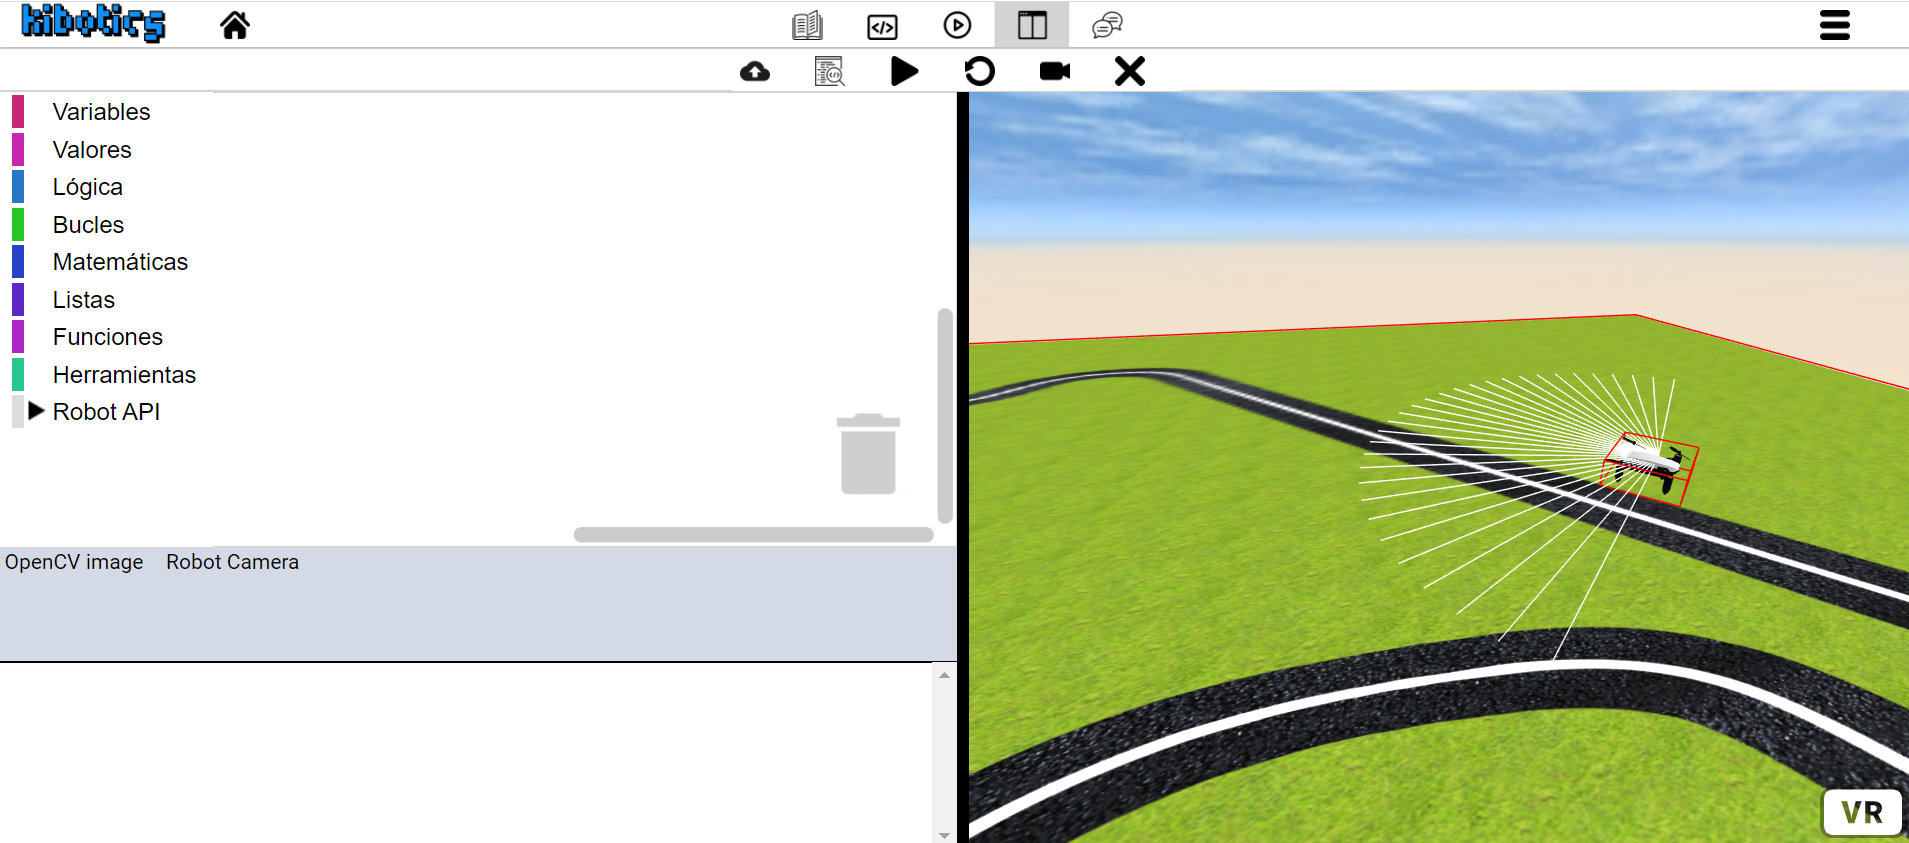
\includegraphics[scale=0.5]{kibotics.PNG}
    \caption{Interfaz de programación en \textit{Kibotics} de un ejercicio en \textit{Scratch}}
    \label{fig:kibotics}
\end{figure}


Todos los robots cuentan con cámaras incorporadas en el hardware, lo que permite la creación de ejercicios que se deben solucionar mediante la utilización de la visión artificial además de los ejercicios que se puedan solucionar mediante el uso de los sensores de los robots (sensores infrarrojos, por ejemplo). La Figura \ref{fig:RobotsKibotics} muestra los robots que soporta actualmente la plataforma.\newline


\begin{figure}[h!]
  \begin{subfigure}[b]{0.2\textwidth}
    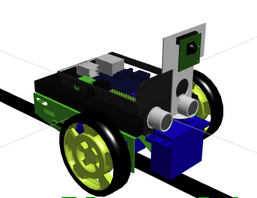
\includegraphics[width=\textwidth, height=\textwidth]{pibot.png}
    \caption{piBot}
  \end{subfigure}
  \hfill
  \begin{subfigure}[b]{0.2\textwidth}
    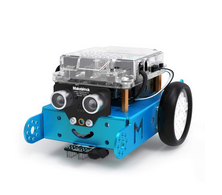
\includegraphics[width=\textwidth, height=\textwidth]{mbot.png}
    \caption{mBot}
  \end{subfigure}
    \hfill
  \begin{subfigure}[b]{0.2\textwidth}
    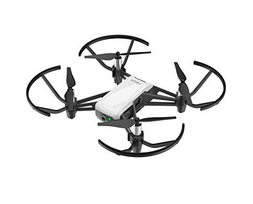
\includegraphics[width=\textwidth, height=\textwidth]{tello_2.png}
    \caption{Drone Tello}
  \end{subfigure}
    \hfill
  \begin{subfigure}[b]{0.2\textwidth}
    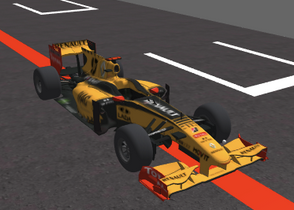
\includegraphics[width=\textwidth, height=\textwidth]{f1.png}
    \caption{Fórmula 1}
  \end{subfigure}
\caption{Robots soportados en la plataforma \textit{Kibotics}}
\label{fig:RobotsKibotics}
\end{figure}


\section{Motores de físicas}
Un motor de físicas es un software capaz de realizar simulaciones de ciertos sistemas físicos como la dinámica del cuerpo en movimiento, la fricción y la elasticidad de una colisión. Se emplean con mucha frecuencia en los videojuegos, para recrear con un mayor realismo el movimiento de los personajes. \newline

Existen numerosos motores de físicas como \textit{Box2D, Cocos2D, Ammo.js o CANNON}. El presente trabajo se va a centrar en este último, ya que es el que emplea \textit{A-Frame} en la actualidad. En el capítulo 3: Herramientas se explicará con mayor detalle las peculiaridades de este motor de físicas en cuestión. \newline

